\section{Region Identification}

Based on the methodology described earlier, we have identified
sections of contigs with one or more overlapping predicted sequences
(features). The result of this processing is a GFF formatted file with
each entry containing information about a region on a specific
contig. Also contained in each entry, is a list of all features
included in that region with start/stop position and strand, the tools
used to predict the features, and a count of how many prediction tools
that were included in said region. Initial analysis of the output is
discussed in this section.

With our results, the first interesting area to look at is simply the
total number of regions identified for any given assembly as well as
number of regions that each tool was a member(weird wording) of. In
figure~\ref{regioncounts}, we see that Braker2 deviates from both the
RefSeq and GeneMark predictions greatly, except in the case of
\textit{T.reesei}. As speculated earlier, this may be due to the
training dataset supplied to Braker2 as it happens to be present in a
similar number of regions when compared to RefSeq and GeneMark in
\textit{T. reesei}. In general, it appears that the RefSeq predictions
are present in more regions than both Braker2 and GeneMark. 

\begin{figure}
  \makebox[\textwidth][c]{
    \begin{tabular}{|c|c|c|c|c|c|c|}
      \hline
      Assembly & Regions (total) & RefSeq & Braker2 & GeneMark \\ \hline
      DC1 & 11268 & NA & 8485 & 11265 \\ \hline
      Tsth20 & 12285 & NA & 8747 & 12279 \\ \hline
      \textit{T. harzianum} & 13377 & 13122 & 8051 & 11529 \\ \hline
      \textit{T. virens} & 12045 & 11864 & 7554 & 11413 \\ \hline
      \textit{T. reesei} & 9818 & 8836 & 9202 & 8897\\ \hline
    \end{tabular}
  }
  \caption{Counts of regions identified in total and total number of
    regions where a prediction from each individual tool was found.}
  \label{regioncounts}
\end{figure}

Figure~\ref{regioncounts} demonstrates that the composition of regions
can differ significantly based on the tools used. To illustrate
agreement of tools in regards to identified regions, Venn diagrams
were generated showing agreement of predictions in a region for each tool.

\begin{figure}
  \centering
  \subfigure[]{\label{fig:a}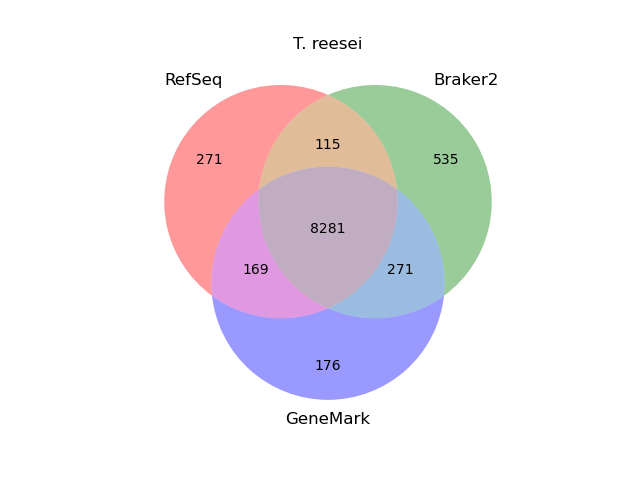
\includegraphics[width=0.45\textwidth]{figures/t-reesei-regions-venn3.png}}
  \subfigure[]{\label{fig:a}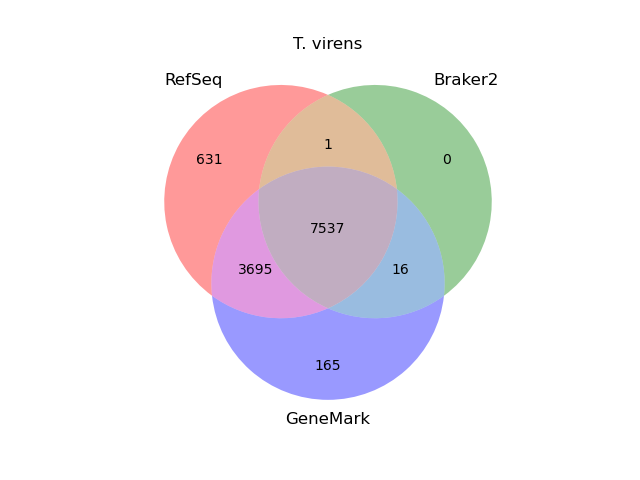
\includegraphics[width=0.45\textwidth]{figures/t-virens-regions-venn.png}}
  \subfigure[]{\label{fig:a}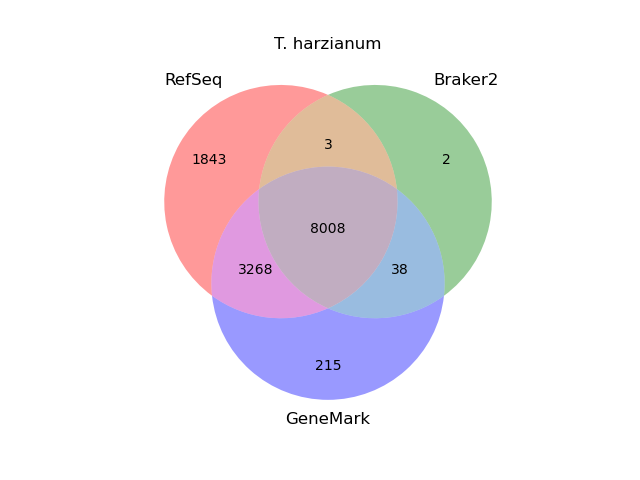
\includegraphics[width=0.45\textwidth]{figures/t-harzianum-regions-venn.png}}
  
\end{figure}

blah blah
